\chapter{Mechanik}

\renewcommand{\kapitelautor}{Autor: Alexander Punz}

\section{Allgemeine technische Planung}

		\subsubsection{Allgemeine Informationen über 3D Drucken}

		Die Technologie des 3D Druckens hat in den letzten Jahren immer mehr an Popularität gewonnen. Mit Hilfe des 3D Druckers kann man fast alle vorstellbaren Formen anfertigen.
		Es gibt verschiedenste Verfahren wie man ein Werkstück anfertigen kann: Laser Sintern, Stereolithographie, Drucken mit flüssigen Materialien, etc.
		In diesem Projekt wird nur die Variante des Druckens mit flüssigen Material verwendet.
		Diese ist kostengünstig \bzw genau genug für die Teile. Wie der Name schon sagt, wird Material in einem Druckkopf geschmolzen und dann Schicht für Schicht auf der Druckplatte aufgetragen.
		Der Druckkopf fährt nur in X und Y Richtung, die Höhe wird mit der Druckplatte selbst verfahren.

		Meist werden Drucker über einen Maschinencode gesteuert, dem sogenannten „G-Code“. In diesem Code werden die Punkte (Koordinaten) definiert, die der Extruder (Druckkopf) abfahren muss.
		Die folgende Abbildung zeigt ein Beispiel eines Maschinencodes.

			\begin{figure}[tbh]
			\begin{centering}
			\includegraphics[width = 0.45\textwidth]{Bilder/gcode_erklaerung}
			\par\end{centering}
			\caption{Maschinencode Erklärung}
			\label{gcode_erklaerung}
			\end{figure}

			% Table generated by Excel2LaTeX from sheet 'Tabelle1'
			\begin{table}[htbp]
  		\centering
  		\caption{Befehle G Code}
	    \begin{tabular}{ll}
	    G1    & Kontrollierte Bewegung \\
	    X, Y  & Koordinaten in horizontaler und vertikaler Richtung \\
	    E     & Angabe der Menge des Filaments, dass in den Extruder geschoben werden muss \\
	    F     & Geschwindigkeit, mit der das Material in den Extruder geschoben wird (mm/min) \\
	    \end{tabular}%
	  	\label{tab:befehle gcode}%
			\end{table}%

		Je nachdem wie der Drucker aufgebaut ist, werden die Produkte genau oder nur grob angefertigt. Sehr genaue Teile kann man am besten in einem Drucker produzieren, der einen geschlossenen Druckraum \bzw eine beheizte Druckplatte hat.
		Besonders an dünnen Platten merkt man das. Wenn der Druckraum nach \bzw während des Druckvorgangs warm ist, kühlt das Werkstück an jeder Stelle fast gleich ab.
		Ist der Druckraum offen, kühlt das Werkstück in der Mitte schneller ab, kühles Material zieht sich zusammen, daher biegt sich das Material auf.

			\newpage

		Es kann vorkommen, dass ein Teil nur so gedruckt werden kann, wenn es nicht komplett auf der Druckplatte aufliegt zum Beispiel ein Steg, der „in der Luft“ liegt oder eine Bohrung im Werkstück, die horizontal gedruckt werden muss.
		In solchen Fällen, druckt der Drucker unter diesem Steg Stützmaterial. Basierend auf diesem Stützmaterial, wird dann die gewünschte Form gedruckt.
		Das Stützmaterial ist so gefertigt, dass man es leicht von dieser abbrechen kann, ohne dass Rückstände zurück bleiben.

		\subsubsection{Materialeigenschaften}

		\subsubsection{Von der Idee zur Anfertigung}

		Die größte Hürde an der Realisierung einer Idee ist, eine CAD Zeichnung zu erstellen. In 3D CAD Programmen wie Creo, SolidWorks, etc. kann man ein Teil konstruieren und dann als STL (Standard Triangulation Language) File abspeichern.
		Dieses Format gibt dann nur mehr Informationen über die Oberfläche und Struktur an (siehe Abbildung\ref{stl_file_optionen}).
		Die Sehnenhöhe gibt an wie genau die Oberfläche gedruckt werden muss, die Winkelsteuerung gibt die Genauigkeit der Radien und Kanten des Teiles an.


			\begin{figure}[tbh]
			\begin{centering}
			\includegraphics[width = 0.5\textwidth]{Bilder/stl_file_optionen}
			\par\end{centering}
	 		\caption{Einstellung für STL File}
			\label{stl_file_optionen}
			\end{figure}

		Mit diesem File kann man anschließend in Programmen wie Slic3r den gewünschten Maschinencode generieren lassen.
		In diesen Programmen gibt man die Lage des Werkstückes an \bzw in genaueren Einstellungen auch die Temperatur des Druckbettes, den Geschwindigkeiten und ähnliche Konfigurationen.

		Am häufigsten haben die Drucker eine USB Schnittstelle, \bzw verfügen über einen SD Karten Slot.
		Der Maschinencode wird auf diesen Speichermedien gespeichert und einfach auf den Drucker überspielt.


\section{Halterung für Cupcakes}

		\subsection{Technische Planung}

		Die Diplomarbeit hat sich speziell auf den Transport von Cupcakes präzisiert, um diesen sicher transportieren zu können, ist es notwendig eine Halterung zu konzipieren.
		Diese Halterung soll möglichst leicht und nicht zu kompliziert zu montieren sein.
		Der Akku wurde an der Unterseite des Hexacopters befestigt, daher war es nur mehr möglich die Halterung an der oberen Centerplate zu platzieren.
		Damit der Multicopter möglichst ausgewogen ist, muss sich das zu transportierende Objekt in der Mitte befinden. Die Idee war es daher, den Cupcake mit einer Halterung zu umranden, damit er nicht verrutschen kann.
		Die Geometrie der Platte \bzw die Größe des Objektes hat die Befestigungsmöglichkeiten stark eingeschränkt (siehe Abbildung \ref{platte_cupcake}).

			\begin{figure}[tbh]
			\begin{centering}
			\includegraphics[width = 0.5\textwidth]{Bilder/platte_cupcake}
			\par\end{centering}
			\caption{Position Cupcake}
			\label{platte_cupcake}
			\end{figure}

		Damit der Cupcake optimal gehalten wird, sollten Stützen entwickelt werden, die in den inneren Rillen der Centerplate befestigt werden.
		Diese Stützen liegen direkt an der Form des Desserts an, um es gegen Verrutschen zu sichern. Die Umsetzung der Planung wird in dem folgenden Punkt erklärt.

			\newpage

	\subsection{Umsetzung}

	Wie schon in der technischen Planung erwähnt wurde, sollte das Objekt von Stützen umrandet werden. Die inneren Ausnehmungen der oberen Centerplate haben sich optimal angeboten, da diese zu der Form des Cupcake reichen.
	Es wurden Stützen konstruiert, die in den Ausnehmungen fixiert werden können und sich direkt an das Dessert anpassen. Die folgenden Abbildungen zeigen die konstruierten Halterungsstutzen und ihre Fixiermöglichkeit.

	\begin{figure}[H]
	  \begin{centering}
	    \subfigure[Halterung Cupcake oben]{\includegraphics[width = 0.4\textwidth]{Bilder/halterung_cupcake_oben_grosz}}
	    \subfigure[Halterung Cupcake unten]{\includegraphics[width = 0.4\textwidth]{Bilder/halterung_cupcake_unten_grosz}} %%%%%%%%%Objekt statt Colorcode
	  \par\end{centering}
	  \caption{Halterung Cupcake}
	  \label{Halterung_Cupcake}
	\end{figure}

	Die Stützen wurden so entworfen, dass sie sich dem Radius \bzw der Höhe der Form des Cupcake anpassen. Die Höhe der Halterung wurde so gewählt, dass etwa die Hälfte der Cupcakeform frei liegt.
	Das soll vermeiden, dass man sich die Finger an der Creme schmutzig machen muss.

	Die Halterung wird mittels Sechskantmutter \bzw Zylinderkopfschrauben festgeschraubt. Aufgrund dessen, dass die Muttern zwischen den zwei Centerplates befestigt werden müssen, wurden die \textcolor{red}{roten} Mutternhalter konstruiert.
	Diese sollen verhindern, dass sich die Muttern beim Festschrauben der Schrauben mitdrehen. Durch diese Halterungen muss man die Muttern nicht mit den Fingern oder einem Gabelschlüssel festhalten.
	Da der Platz sehr begrenzt ist, überlappen sich die zwei Schrauben \bzw die Muttern, aufgrund dieses Problems wurden Höhenunterschiede zwischen den Schraubenköpfen \bzw der Sechskantmuttern eingeplant.

		\newpage

	\subsection{Herausforderungen und Lösungen}

	Die größte Herausforderung am Konstruieren war es, die Halterung exakt an die Form des Cupcakes anzupassen. Die Rundung in der Halterung sollte genau an die Kegelform des Cupcakes passen.
	Um dieses Problem zu lösen, wurde der exakte Mittelpunkt der Centerplate ermittelt. Von diesem Mittelpunkt aus, wurden dann alle Maße gemessen, die benötigt wurden.
	Der Durchmesserverlauf der Form wurde mit Winkelfunktionen errechnet und dann an die Halterung angepasst.

	Wie schon erwähnt, war der Platz für Befestigungsschrauben sehr eingeschränkt. Die großen Toleranzen des Druckers haben die Konstruktion sehr beeinflusst.
	Da manche Bohrungen nur sehr dünne Wände haben, brachen diese beim Drucken ein oder wurden nur sehr grob gefertigt. Die folgende Abbildung zeigt die Halterungen an dem Hexacopter befestigt.

		\begin{figure}[tbh]
		\begin{centering}
		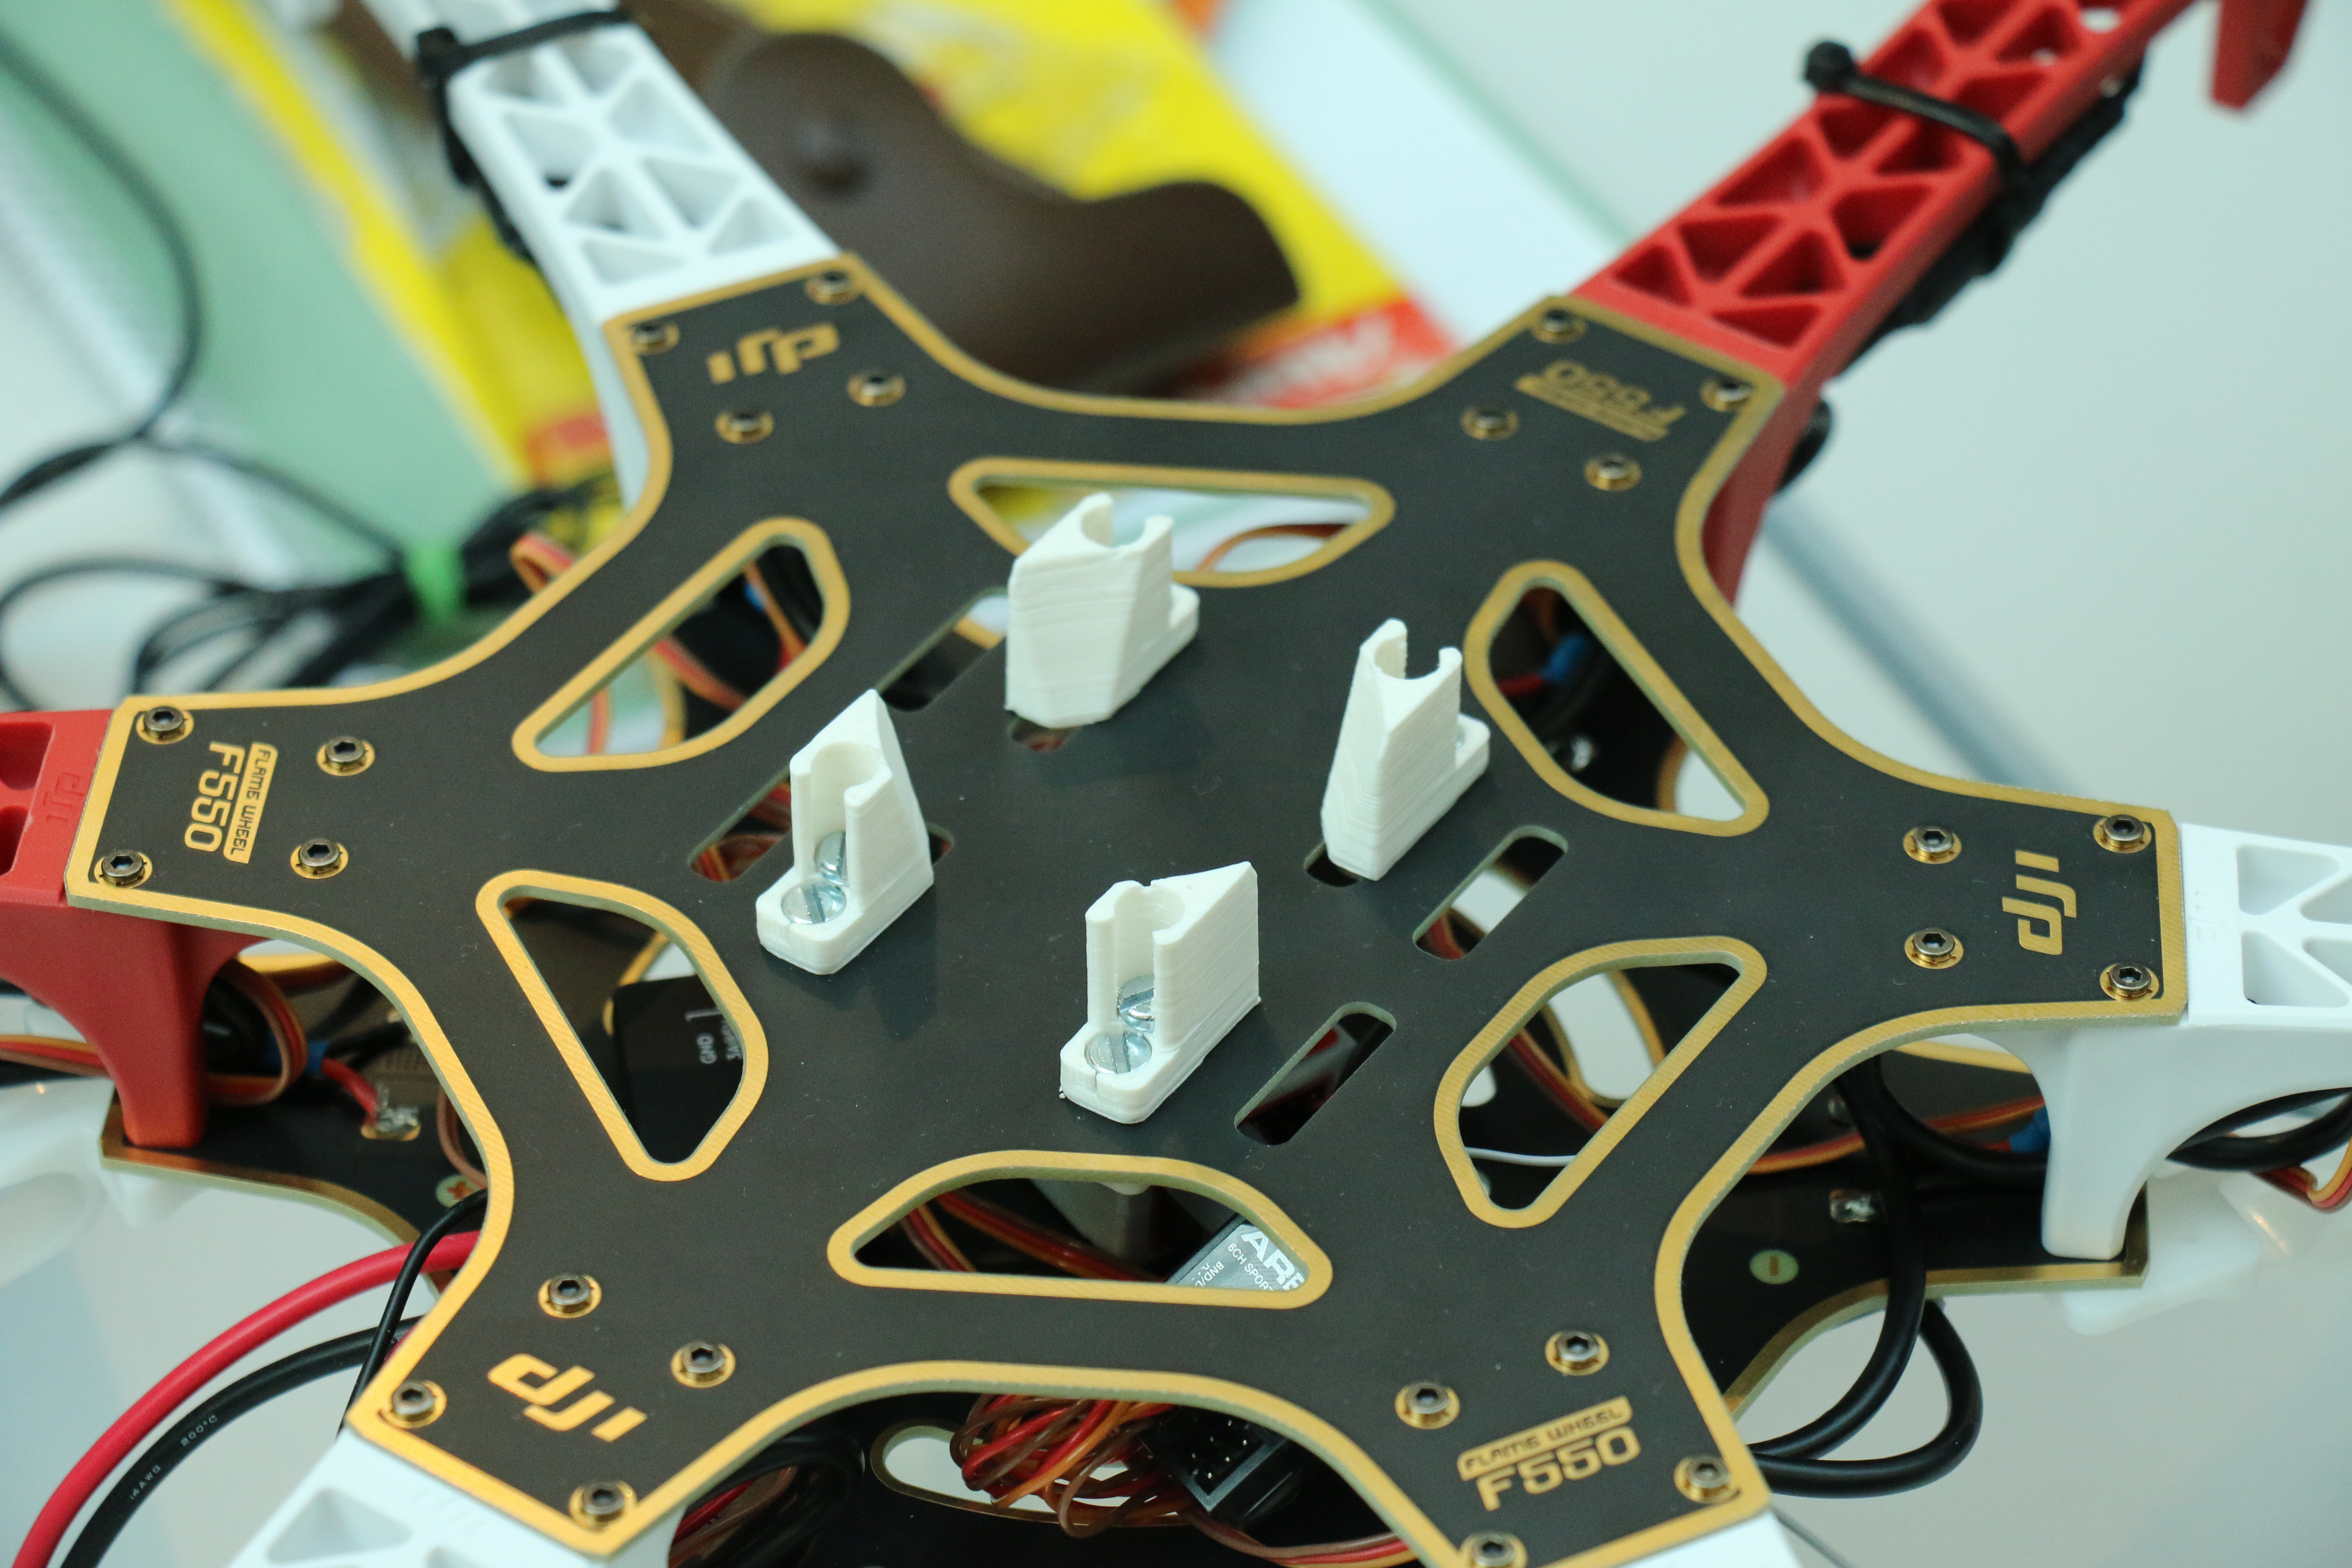
\includegraphics[width = 0.65\textwidth]{Bilder/halterung_cupcake_fertig}
		\par\end{centering}
		\caption{Gedrucktes Halterungssystem}
		\label{halterung_cupcake_fertig}
		\end{figure}

		Wie man an manchen Stellen der Stützen erkennen kann, sind die Wände leicht eigerissen, jedoch kann man dies nicht verhindern.
		Die Langlöcher der Centerplate sind nur so kurz, dass man die Schrauben nicht weiter nach hinten versetzen kann, um die Wände dicker machen zu können.

		%\subsection{Implementierung}

\section{Rotorschutz}

	\subsection{Technische Planung}

	\subsection{Umsetzung}

	\subsection{Herausforderungen und Lösungen}

	\subsection{Implementierung}

\section{Halterung Ultraschallsensor}

	\subsection{Technische Planung}

	\subsection{Umsetzung}

	\subsection{Herausforderungen und Lösungen}

\section{Halterung PIXY CMU cam5}

	\subsection{Technische Planung}

		\subsubsection{Berechnungen}

	\subsection{Umsetzung}

	\subsection{Implementierung}

	\subsection{Testphase}

\section{Führung für Testflüge}

	\subsection{Technische Planung}

	\subsection{Umsetzung}

	\subsection{Implementierung}

	\subsection{Testphase}

\section{Persönliche Erfahrungen}
